\documentclass[final,hyperref={pdfpagelabels=false}]{beamer}
\usepackage{grffile}
\mode<presentation>{\usetheme{drexel}}

\usepackage[english]{babel}
\usepackage{verbatim}
\usepackage[latin1]{inputenc}
\usepackage{amsmath,amsthm, amssymb, latexsym}
\usefonttheme[onlymath]{serif}
\usepackage{epstopdf}
\epstopdfsetup{update}

%% You can change the poster orientation (portrait vs. landscape) and the paper size (a0, a1, &c.) here:
%\usepackage[orientation=portrait,size=a0,scale=1.4,debug]{beamerposter}
\usepackage[orientation=portrait,size=custom,width=60.96,height=91.44,scale=1]{beamerposter}
\usepackage{array,booktabs,tabularx}
\newcolumntype{Z}{>{\centering\arraybackslash}X} % centered tabularx columns
\newcommand{\pphantom}{\textcolor{ta3aluminium}} % phantom introduces a vertical space in p formatted table columns??!!

\title{\huge Network Alignment}
\author{\Large Nil Mamano\\Advisor: Wayne Hayes, Department of Computer Science}
\email{\texttt{nmamanog@uci.edu}}
\institute[University of California Irvine]{Donald Bren School, UC Irvine}
\date[November 17th, 2015]{November 17th, 2015}

%% Uncomment the following line to define a custom logo (or to tweak the size of the logo
\DrexelLogo{}

%%%%%%%%%%%%%%%%%%%%%%%%%%%%%%%%%%%%%%%%%%%%%%%%%%%%%%%%%%%%%%%%%%%%%%%%%%%%%%%%%%%%%%
\newlength{\columnheight}
\setlength{\columnheight}{105cm}

%%%%%%%%%%%%%%%%%%%%%%%%%%%%%%%%%%%%%%%%%%%%%%%%%%%%%%%%%%%%%%%%%%%%%%%%%%%%%%%%%%%%%%
\begin{document}

\begin{frame}
  \noindent\begin{columns}
    % ---------------------------------------------------------%
    % Set up a column 
    \begin{column}{.49\textwidth}
      \begin{beamercolorbox}[center,wd=\textwidth]{postercolumn}
        \begin{minipage}[T]{.95\textwidth}  % tweaks the width, makes a new \textwidth
          \parbox[t][\columnheight]{\textwidth}{ % must be some better way to set the the height, width and textwidth simultaneously
            % Since all columns are the same length, it is all nice and tidy.  You have to get the height empirically
            % ---------------------------------------------------------%
            % fill each column with content            
            \begin{block}{Introduction}

Network alignment is the task of finding the best way to ``fit'' one network inside another. It has applications in several
areas, such as language processing and social networks. We focus on a particular application from the computational biology domain:
the alignment of protein-protein interaction (PPI) networks. In a PPI network, nodes represent proteins from a given organism, and edges connect proteins that interact physically.

PPI networks can have thousands of nodes and tens of thousands of edges.
\begin{figure}
\centering
\includegraphics[width=0.68\linewidth]{../figures/proteinmap}
\caption{Yeast PPI Network.}
\label{fig:proteinmap}
\end{figure}

Aligning PPI networks of different species has many interesting applications. It can serve to transfer biological information across species, which, in turn, has been used to offer insights on the mechanisms of human diseases, or the process of aging in humans.

            \end{block}
            \vspace{50px}
%\begin{verbatim}
 
 
 
%\end{verbatim}
            \begin{block}{Problem Description}

Our goal is to compare PPI networks of different species by aligning their nodes. An alignment is a mapping between the nodes in both networks.
We would like to find the most biologically relevant mapping: aligned proteins should come from the same protein in the species which was the common ancestor of the species of both PPI networks.

\begin{figure}
\centering
\includegraphics[width=0.6\linewidth]{../figures/net_align}
\caption{Alignment between two networks. One is colored in red
(nodes) and orange (edges), while the other graph is colored in white (nodes) and gray
(edges). The alignment is colored in blue.}
\label{fig:net_align}
\end{figure}

In order to create the alignments, we look at the networks' topology. We try to maximize the number of edges conserved by the alignment:

\begin{figure}
\centering
\includegraphics[width=0.9\linewidth]{../figures/conservededges}
%\caption{}
\label{fig:conservededges}
\end{figure}

The number of conserved edges is only one of many criteria of alignment ``quality'', called \textit{evaluation functions}. Part of our work consisted on doing a survey and classification of evaluation functions, and even proposed some new ones.
            \end{block}
          }
        \end{minipage}
      \end{beamercolorbox}
    \end{column}
    % ---------------------------------------------------------%
    % end the column

    % ---------------------------------------------------------%
    % Set up a column 
    \begin{column}{.49\textwidth}
      \begin{beamercolorbox}[center,wd=\textwidth]{postercolumn}
        \begin{minipage}[T]{.95\textwidth} % tweaks the width, makes a new \textwidth
          \parbox[t][\columnheight]{\textwidth}{ % must be some better way to set the the height, width and textwidth simultaneously
            % Since all columns are the same length, it is all nice and tidy.  You have to get the height empirically
            % ---------------------------------------------------------%
            % fill each column with content
            
            
            
            
            \begin{block}{The Algorithm}

We use an algorithm called Simulated Annealing to find an alignment maximizing EC, the number of conserved edges (or any other objective function). This algorithm starts with a random alignment, and gradually improves it by \textbf{changing} and \textbf{swapping} assignments.

\begin{figure}
\centering
\includegraphics[width=0.55\linewidth]{../figures/operatorssimplified}
%\caption{}
\label{fig:operatorssimplified}
\end{figure}             
              
If we repeat this process, we will
reach a \textit{local maximum} in which we can no longer improve. However, this local maximum is unlikely to be the best overall solution. To avoid this pitfall, Simulated Annealing introduces the ability to allow worse solutions to be selected with some probability. This probability starts high and decreases towards zero. Our experiments suggest that the results best when it decreases slowly.
\begin{figure}
\centering
\includegraphics[width=0.57\linewidth]{../figures/tempschedule}
\caption{Fraction of conserved edges (EC) as a function of time for different values of $\lambda$, the parameter that controls how quickly the probability to accept a worse solution decreases.}
\label{fig:tempschedule}
\end{figure}             
            
            \end{block}
            \vspace{20px}
      %      \vfill
            \begin{block}{Results}

Our method SAGA (Simulated Annealing Graph Aligner) improves significantly over all previous work, on the three datasets we used and for all evaluation functions. Moreover, it is among the fastest methods.
              
\begin{figure}
\centering
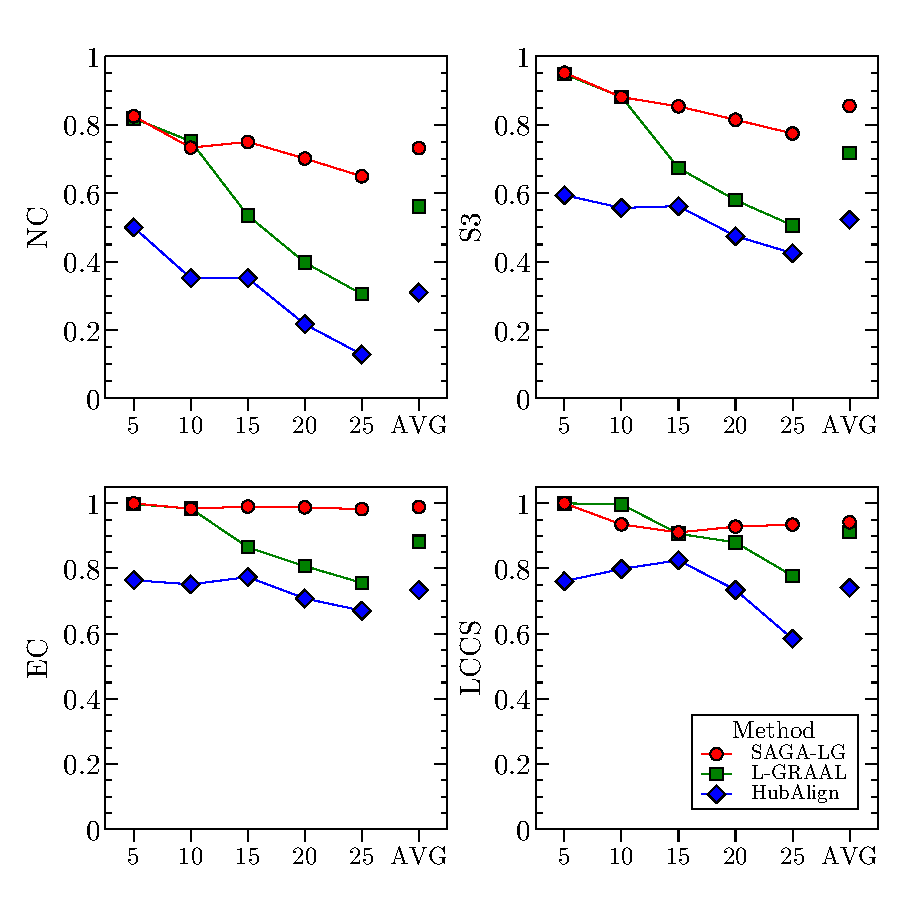
\includegraphics[width=0.7\linewidth]{../sanaPaper/syntheticyeast_bw.eps}
\caption{Comparison of SAGA with L-GRAAL and HubAlign, two of the best-performing network alignment methods. Since in SAGA we can choose which objective function to optimize, we chose the same objective function that L-GRAAL uses to make a more direct comparison. In the plot we call this variation SAGA-LG. We align the Yeast PPI network to noisy versions of itself: the $x$-axis denotes the $\%$ of noise added. The comparison includes four evaluation functions. The most important is \textit{Node correctness} (NC), which is the fraction of nodes assigned to themselves in the noisy network. The others are Edge Conservation (EC), Symetric Substrcture Score (S3), and Largest Common Connected Subgraph (LCCS).}
\label{fig:syntheticyeastresults}
\end{figure}                

            \end{block}
%            \vfill
%
 %           \begin{block}{Conclusions}
%
 %             Nulla ultrices, mauris quis venenatis pretium, est odio
%
 %           \end{block}
          }
          % ---------------------------------------------------------%
          % end the column
        \end{minipage}
      \end{beamercolorbox}
    \end{column}
    % ---------------------------------------------------------%
    % end the column
  \end{columns}
\end{frame}
\end{document}


%%%%%%%%%%%%%%%%%%%%%%%%%%%%%%%%%%%%%%%%%%%%%%%%%%%%%%%%%%%%%%%%%%%%%%%%%%%%%%%%%%%%%%%%%%%%%%%%%%%%
%%% Local Variables: 
%%% mode: latex
%%% TeX-PDF-mode: t
%%% End: